
\documentclass[twocolumn, a4paper]{ieicejsp}
\usepackage{newenum}
\usepackage[dvipdfmx]{graphicx}
\usepackage{latexsym}
\usepackage{amsmath}
\usepackage{amssymb}
\usepackage{multirow,eepic}
\usepackage{cite}
\usepackage{mediabb}
\usepackage{url}
\usepackage{comment}
\usepackage{epsfig}
\usepackage{subfig}

\newcommand{\sij}{(i,\ j)}
\newcommand{\mN}{{\mathcal N}}
\newcommand{\pij}{p^{(i,\ j)}}
\newcommand{\rd}{r^{\sij}_{\rm d}}
\newcommand{\ru}{r^{\sij}_{\rm u}}
\newcommand{\rij}{r^{\sij}}
\newcommand{\etau}{\eta_{\rm u}^{(j)}}
\def\coloneqq{\mathrel{\mathop:}=}

\title{{\bf 全二重通信無線LANにおける端末組み合わせ決定手法の検討}
  {\normalsize \\Station Pairing Scheme for In-Band Full-Duplex Wireless LANs}}
  \author{
    飯田 直人\\ Naoto Iida
  }
  \affliate{
    京都大学大学院 情報学研究科 通信情報システム専攻 守倉研究室
    }

\begin{document}
\maketitle
\section{はじめに}
	近年,無線LAN(Local Area Network)システムの大容量化を実現する方法の一つとして,
	送信と受信を同じ周波数帯で同時に行う全二重通信無線LANが注目されており,
	理想的には無線LANの通信容量を2倍にすることができる.
	本稿では図\ref{fig:topology}に示すような上り通信を行うSTAと下り通信を受信するSTAが異なる全二重通信
	(UFD: user-multiplexing Unidirectional Full-Duplex)を扱う.
	このUFD通信を用いた無線LANでは二つの干渉が問題となる.
	一つは,送受信を行っているAPにおいて送信信号が所望の受信信号に干渉を及ぼす自己干渉であるが,
	自己干渉除去技術を用いて自己干渉を最大110\,dB除去できることが示されている~\cite{stanford1}.
	もう一つは,STA $j$の送信信号がもう一方のSTA $i$の受信信号に干渉を及ぼすユーザ間干渉である.
	ユーザ間干渉は自己干渉のように除去することができない.
	このユーザ間干渉の影響を低減するためには,干渉の大きさを考慮して適切なSTA $i$,$j$の組み合わせを選び出すことや,
	送信電力制御を行うことが必要である.
	\cite{promac}では,STAの組み合わせ毎の干渉量から合計スループットを推定し,
	その値を最大化するSTAの組み合わせを確率的に選択する方式を提案している.
	\par
	しかし,これらのMAC(Media Access Control)プロトコルでは極端に条件の良いSTAが存在すると組み合わせの選択に大きく偏りを生じ,公平性が低下する.
	加えて,QoS(Quality of Service)制御に関する議論はなされておらず,
	例えば音声通話などの低遅延を要求するアプリケーションサービスを利用するSTAに対しても干渉量やスループットを基準にSTAを選択するため,
	送信機会が得られず遅延が大きくなる可能性がある.
	\par
	本稿では,既存研究~\cite{promac}で議論される確率的なSTA選択手法を用いたMACプロトコルをもとに,
	STA間の送信機会の公平性を改善するための目的関数とSTA毎の遅延要求に応じたQoS制御手法に関して提案する.
	更に,本手法の有効性を計算機シミュレーションにより評価する.

	\begin{figure}[t]
		\centering
		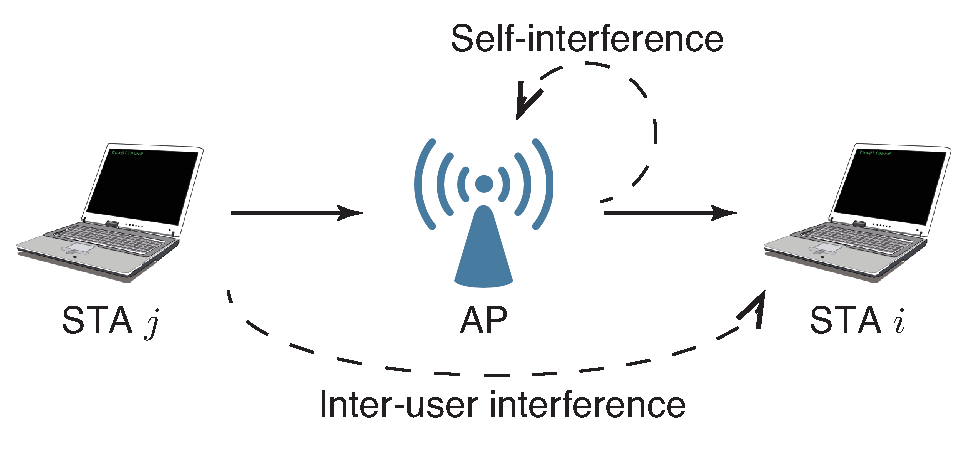
\epsfig{file=fig/model_relay.eps, scale=0.4}
		\caption{UFDにおける自己干渉とユーザ間干渉}
		\label{fig:topology}
	\end{figure}
\section{システムモデル}
	\begin{figure}[t]
		\centering
		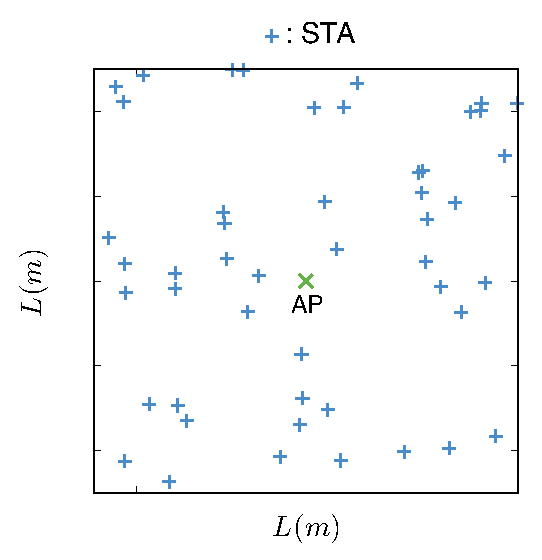
\epsfig{file=fig/pos.eps, scale=0.6}
		\caption{システムモデル(中心に設置されたAPとランダムに配置されたSTA)}
		\label{fig:model}
	\end{figure}

	本稿で検討するシステムモデルを図\ref{fig:model}に示す.
	1台のAPが$L$\,m四方の領域の中心に設置され,その周りに$N$台のSTAがランダムに配置されているとする.
	それらSTAのインデックス集合を$\mN=\{1,2,...,N\}$とする.
	この$N$台のSTAの中から,図\ref{fig:topology}のようにAPからの下り通信を受信するSTA $i$と,
	APへの上り通信を行うSTA $j$を選び出す.
	このとき,STAの組み合わせを$\sij$と表現し,$i,\ j \in \{0\}\cup \mN$であり,
	STAは自己干渉除去技術を持たずBFD通信はできないと仮定して$i\neq j$とする.
	ただし,$i=0$のときは下り通信を伴わない上り通信のみの半二重通信であり,
	$j=0$のときは上り通信を伴わない下り通信のみの半二重通信であるとする.
	更に,この$N$台のSTAの中に低遅延を要求するアプリケーションサービスを用いているSTAが存在し,
	そのインデックス集合を${\mathcal D}\subset\mN$とする.
	ただし,低遅延を要求しないSTAのインデックス集合は${\overline {\mathcal D}}\coloneqq{\mathcal N}/{\mathcal D}$とする.
	また,STAの組み合わせを決定する際に用いる実効スループットには,上り下り通信のそれぞれのSINR(Signal-to-Interference plus Noise power Ratio)から求めた以下のシャノン容量$C$を用いる.
	\begin{equation}
		C=B\log_2(1+{\rm SINR}) \label{eq:capacity}
	\end{equation}
	ただし,$B$は通信に用いる帯域幅である.

\section{既存研究}
	本章では従来方式~\cite{promac}のMACプロトコルについて述べる.
	このMACプロトコルはシステムスループットの期待値を目的関数とし,
	各STAの組み合わせの選択確率を変数とした最適化問題を解くことで各STAの選択確率を決定し,確率的なSTA選択を行う.
	\subsection{STAの組み合わせの決定手順}\label{sec:promac}
		このMACプロトコルでは,APとSTA $i$,$j$の組み合わせで全二重通信が行われる確率$\pij$に基づいてSTA $i$,$j$が決定される.
		\par
		まず,UFD通信を行うSTAの組み合わせの集合${\mathcal C}_{\rm full}$を式\eqref{eq:cfull}に示す.
		\begin{equation}
			{\mathcal C}_{\rm full} \coloneqq \{\sij : i,j\in{\mathcal N},\ i\neq j,\ r^{\sij}_{\rm d},\ r^{\sij}_{\rm u}>\epsilon\} \label{eq:cfull}
		\end{equation}
		ただし,$r_{\rm d}^{\sij}$,$r_{\rm u}^{\sij}$はそれぞれAPからSTA $i$への下りの実効スループット,
		STA $j$からAPへの上りの実効スループットであり,$\epsilon$はスループットが0に近くなるようなSTAの組み合わせを除くためのしきい値である.
		${\mathcal C}_{\rm full}$の全組み合わせに対して,上下通信の実効スループット$\rd$,$\ru$を推定し,$\rij=\rd + \ru$とする.
		ただし,本稿では実効スループットの推定には式\eqref{eq:capacity}を用いる.
		実行スループットの推定には干渉の影響が含まれ,干渉が小さいほど$\rij$は大きくなる.
		更に,半二重通信の組み合わせ
		\begin{equation}
			{\mathcal C}_{\rm half} \coloneqq \{\sij : ij=0,\ \rij >\epsilon\}
		\end{equation}
		に対しても実効スループット$\rij$を推定する.
		得られた$\rij$に基づいて以下の最適化問題を解き,確率$\pij$を得る.
		\begin{align}
			&{\mathcal P}_1: && {\rm max} \sum_{(i,\ j)\in{\mathcal C}} p^{(i,\ j)}r^{(i,\ j)} &&&&&& \label{eq:p1}\\
			&{\rm subject\ to} && \sum_{j\in\{j:(i,\ j)\in{\mathcal C}\}} p^{(i,\ j)} \geq \eta_{\rm d}^{(i)},\ \forall i\in {\mathcal N}  \\
			&&& \sum_{i\in\{i:(i,\ j)\in{\mathcal C}\}} p^{(i,\ j)} \geq \eta_{\rm u}^{(j)},\ \forall j\in {\mathcal N} \label{eq:pu}\\
			&&& \sum_{j\in\{j:(i,\ j)\in{\mathcal C}\}} p^{(i,\ j)}=1 \\
			&{\rm variables:} &&p^{(i,\ j)} \in {\mathbb R}_{\geq 0},\ \forall(i,\ j)\in {\mathcal C} \nonumber
		\end{align}
		ただし,${\mathcal C} = {\mathcal C}_{\rm full} \cup {\mathcal C}_{\rm half}$である.
		実行スループット$\rij$は干渉が小さいほど大きくなり,大きい$\rij$を持つSTAの組み合わせほど$p^{\sij}$が大きくなる.
		$\eta_{\rm d}^{(i)}$はSTA $i$が下り通信の送信先となる確率$p_{\rm d}^{(i)}=\sum_{j\in\{j:(i,\ j)\in{\mathcal C}\}} p^{(i,\ j)}$
		の最低値であり,STA $i$への下り通信のトラヒックに比例した値が設定される.
		同様に,$\eta_{\rm u}^{(j)}$は$p_{\rm u}^{(j)}=\sum_{i\in\{i:(i,\ j)\in{\mathcal C}\}} p^{(i,\ j)}$
		の最低値であり,STA $j$の上り通信のトラヒックに比例した値が設定される.
		また,以下の条件が満たされるとき必ず解が得られることが示されている.
		\begin{align}
			r_{\rm d}^{(i,\ 0)} >\epsilon,\ \forall i\in\mN \\
			r_{\rm u}^{(0,\ j)} >\epsilon,\ \forall j\in\mN \\
			\sum_{i\in\mN}\eta_{\rm d}^{(i)} + \sum_{j\in\mN}\eta_{\rm u}^{(j)} =1 \label{eq:feasible}
		\end{align}
		なお,この最適化問題は毎回あるいは複数のビーコン信号周期毎に解かれ,更新された確率$\pij$はビーコンフレームによってSTAに通知される.
		\par
		次に,得られた$\pij$を用いてSTA $i$,$j$を決定する方法を述べる.
		APは
		\begin{equation}
			p_{\rm d}^{(i)}= \sum_{j\in\{j:(i,\ j)\in{\mathcal C}\}}p^{(i,\ j)},\ \forall i \in \{0\}\cup{\mathcal N}
		\end{equation}
		によって各STAが下り通信の送信先となる確率$p_{\rm d}^{(i)}$を求め,$p_{\rm d}^{(i)}$に従って確率的に送信先STA $i$を選択する.
		続いてSTA $j$の上り通信の送信権について述べる.
		APからの下り通信を受信するSTA $i$の決定後,APはSTA $i$へ送信するフレームのヘッダ部分のみを送信し,
		全STAに下り通信の送信先がSTA $i$であることを通知する.
		STA $i$以外のすべてのSTAは以下の条件付き確率
		\begin{equation}
			p_{\rm u}^{\sij} = P(j\ {\rm wins\ uplink}\mid{\rm AP\ sends\ to}\ i)=\pij / p_{\rm d}^{(i)} \label{eq:win}
		\end{equation}
		を計算する.
		これはAPがSTA $i$へ下り通信を行うことが決まった上で自身がAPへの上り通信の送信権を獲得する確率を意味する.
		この条件付き確率をもとに,コンテンションウィンドウサイズ${\rm CW}^{\sij}_{\rm u}$を
		\begin{equation}
			{\rm CW}^{\sij}_{\rm u} = \lceil 1/p_{\rm u}^{\sij} \rceil
		\end{equation}
		と設定する.
		ただし,$\lceil x \rceil$は$x$を超えない最大の整数である.
		各STAは$[0,\ {\rm CW}^{\sij}_{\rm u}]$の一様分布から生成されるバックオフカウンタ$w_{\rm u}^{\sij}$を設定し,
		CSMA/CAのバックオフアルゴリズムを用いてバックオフカウンタを1ずつ減らす.
		その結果,最初にカウンタが0となったSTAが上り通信を行う.
		この方法により,$p_{\rm u}^{(j)}$が大きいSTA,つまり式\eqref{eq:p1},\eqref{eq:win}より$r^{\sij}$が大きいSTAほど${\rm CW}^{\sij}_{\rm u}$が小さくなり,送信権を得やすくなる.

	\subsection{課題}
		式\eqref{eq:p1}からわかるように~\cite{promac}では,STA $i$,$j$の干渉が小さくスループット$\rij$が大きい組み合わせほど選ばれる確率が高くなる.
		図\ref{fig:numtx}にSTA台数を$N=50$としたシステムで
		従来方式による各STAの上り通信送信回数のシミュレーション結果を示す.
		この結果から一部のSTAが上り通信を行うSTAになる確率が高く,送信回数が突出して多くなり,
		送信機会に関する公平性は低くなっていることがわかる.
		加えて,STA間の遅延要求の違いについては議論されておらず,低遅延を要求するSTAが混在し
		そのSTAの実効スループットが低い場合,
		そのSTAが送信機会を得るまでに大きな遅延が生じる可能性がある.
		本稿では,この2つの問題点に関して解決を図り,QoSの向上を目指す.

		\begin{figure}[t]
			\centering
			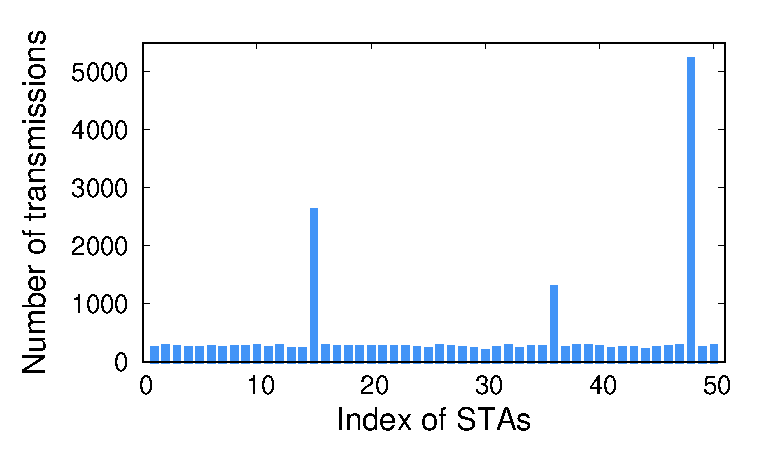
\epsfig{file=graph/numtx.eps, scale=0.6}
			\caption{従来方式によるSTAの送信回数の分布}
			\label{fig:numtx}
		\end{figure}

\section{提案方式}
	\subsection{公平性の改善}\label{sec:fair}
		前節に述べたように従来方式のMACプロトコルでは干渉が小さい組み合わせが選ばれやすく,
		特定のSTAに送信機会が偏るという課題がある.
		この問題を解決をするため以下の目的関数を提案する.
		\begin{equation}
			{\mathcal P}_2: {\rm max} \sum_{(i,\ j)\in{\mathcal C}} p^{(i,\ j)}r^{(i,\ j)}(d^{(j)})^{\alpha} \label{eq:p2}
		\end{equation}
		$d^{(j)}$は待機時間であり,STA $j$のバッファの先頭にフレームが到着してから現在時刻までの時間とする.
		この待機時間の項を追加することで,待機時間が長いSTA,つまり,送信機会を得られていないSTAを含んだ組み合わせが選ばれる確率が高くなり,
		送信機会の均等化を図ることができる.
		また,待機時間は飽和トラヒックである限りは前回の送信時刻からの経過時間と同じであるため,
		新たに各STAの待機時間情報を収集する必要はなく,APが各STA毎に最新の送信時刻を記憶することで,
		現在時刻との差として得られる.
		追加する項として各STAの平均送信間隔や送信回数そのものを選択しない理由は,
		両者はいずれも積算値であるため,新たにSTAがAPに接続された場合平均送信間隔は定義できず,
		送信回数は0であるため選択される確率が極端に高くなり短期的な不公平性が生じる可能性があるためである.
		\par
		公平性の改善を行うと,公平性の改善を行わない場合に比べて比較的干渉の多いSTAの組み合わせが選ばれることが多くなり,
		システムスループットの低下が考えられる.
		そのため,公平性の改善とシステムスループットの低下のトレードオフを調整可能とするための重み係数$\alpha\geq 0$を導入する.
		$\alpha$が小さい場合は待機時間$d^{(j)}$の影響が小さくなるため,システムスループットが高くなり公平性は低くなる.
		逆に$\alpha$が大きい場合は待機時間$d^{(j)}$の影響が大きくなり,システムスループットが大きく低下するかわりに公平性が高くなる.

\section{シミュレーション評価}
	本章では提案手法の有効性をシミュレーションによって評価する.
	図\ref{fig:model}のように,1台のAPが$L$\,m四方の領域の中心に設置され,その周りに$N$台のSTAがランダムに配置されているとする.
	MACプロトコルは~\cite{promac}に従い,従来の目的関数,及び,$\etau$設定法を用いたものと提案の目的関数,及び,$\etau$設定法を用いたものを比較する.
	上下通信ともに飽和トラヒックの場合を取り扱う.

	\begin{table}[t]
		\centering
		\caption{シミュレーション諸元}
		\label{tab:param}
		\begin{tabular}{cc} \hline
			領域の大きさ $L$ & 100\,m \\
			伝送速度 & シャノン容量 \\
			送信電力 & 15\,dBm \\
			雑音指数 & 10\,dB \\
			周波数帯 $f$& 2.4\,GHz \\
			帯域幅 $B$ & 20\,MHz \\
			伝搬損失 & $20\log f+30\log d - 28$\\
			&($d$: 送受信点間距離)\\
			自己干渉除去 & 110\,dB \\
			シミュレーション時間 & 10\,s \\\hline
		\end{tabular}
	\end{table}

	\subsection{公平性の改善}
		図\ref{fig:fair}にSTA台数を$N=50$とした場合の各STAの全シミュレーション時間内での上り通信送信回数を示す.
		図\ref{fig:numtx}と比較して,一部のSTAが極端に選ばれやすいという現象が改善されていることがわかる.
		図\ref{fig:thr_fair}にシステムスループットとSTA間の公平性を示す.
		ただし,結果は10種類の異なるSTA配置によるシミュレーション結果の平均値であり,
		公平性はJain's fairness index~\cite{jain}における各STAのスループットを送信回数に置き換えたもので評価した.
		また,$\alpha=0$は従来方式の結果とする.
		提案方式は$\alpha$を適切に設定することで,従来方式と比較してSTA間の送信機会に関する公平性を大きく改善できることを示した.
		更に,提案方式において重み係数$\alpha$を変化させることで,公平性の改善とシステムスループット低下のトレードオフを調整可能であることを示した.
		また,本シミュレーションでは$\alpha\leq0.4$のときに従来方式と比較してシステムスループットの低下が小さく,公平性が高くなっている.

		\begin{figure}[t]
			\centering
			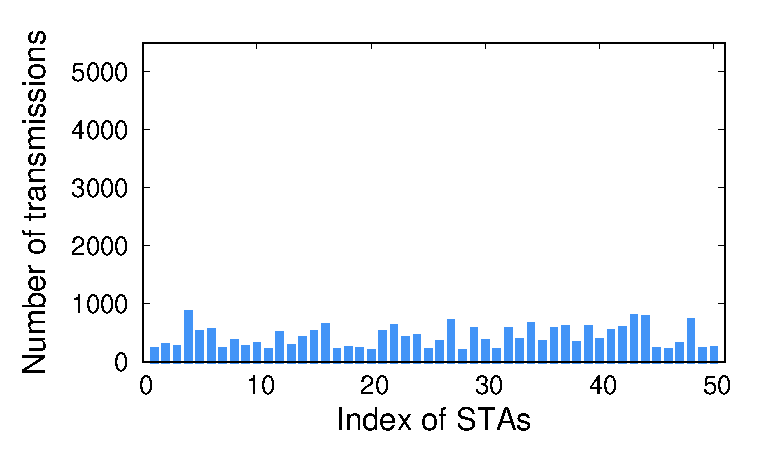
\epsfig{file=graph/numtxfair.eps, scale=0.6}
			\caption{提案方式によるSTAの上り通信送信回数の分布}
			\label{fig:fair}
		\end{figure}

		\begin{figure}[t]
			\centering
			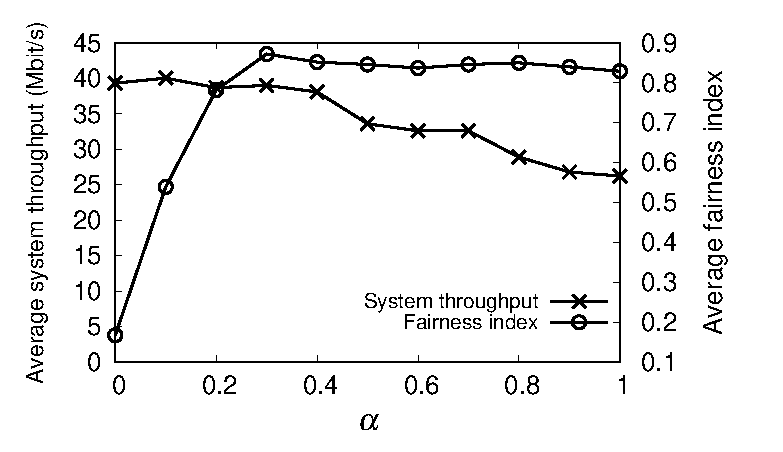
\epsfig{file=graph/thr_fair.eps, scale=0.6}
			\caption{重み係数$\alpha$に対するシステムスループットとfairness index}
			\label{fig:thr_fair}
		\end{figure}

\section{まとめ}
	本稿では,全二重通信無線LANにおけるSTAの組み合わせ選択において,STA間の公平性とQoS制御を行う手法を提案した.
	各STAの送信待機時間を目的関数に組み込み,送信機会を得ることができていないSTAに送信機会を与えることで
	STA間の公平性を大幅に改善した.
	更に,重み係数$\alpha$によって公平性の改善とシステムスループットの低下のトレードオフを調整できることを示した.
	また,低遅延を要求するSTAの送信確率を向上させる制約条件を設計し,QoSの改善を行った.

\bibliographystyle{sieicej}
\bibliography{main2}

\end{document}
